\documentclass[10pt,journal,compsoc,onecolumn]{IEEEtran}
\usepackage[utf8]{inputenc}
\usepackage{amsmath,amsfonts,amssymb}
\usepackage{amsthm}
\usepackage{graphicx}
\usepackage{cite}
\usepackage{textcomp}
\usepackage{tikz}
\usetikzlibrary{arrows,positioning,shapes.geometric}
\usepackage{booktabs}
\usepackage{url}

\newtheorem{theorem}{Theorem}
\newtheorem{lemma}[theorem]{Lemma}
\newtheorem{definition}[theorem]{Definition}
\newtheorem{corollary}[theorem]{Corollary}

\begin{document}

\title{On the Algorithmic and Mathematical Foundations of Combinatorics: A Formal Analysis of the Binomial Theorem, Multinomial Theorem, and Pascal's Triangle}

\IEEEtitleabstractindextext{%
\begin{abstract}
This paper presents a formal analysis of the fundamental principles of combinatorics, focusing on Pascal's Triangle, the Binomial Theorem, and the Multinomial Theorem. We explore the recursive mathematical properties of Pascal's Triangle, formulate the algebraic expansion of binomial and multinomial expressions, and discuss their critical applications in algorithmic design, probabilistic analysis, and dynamic programming optimization. Complete Java reference implementations are provided for efficient algorithmic generation.
\end{abstract}

\begin{IEEEkeywords}
binary trees, algorithms, data structures, computational complexity, tree traversal, recursive algorithms, formal analysis
\end{IEEEkeywords}
}

\maketitle
\IEEEdisplaynontitleabstractindextext
\IEEEpeerreviewmaketitle

\section{Introduction}
\label{sec:intro}

Combinatorics serves as the bedrock of theoretical computer science, discrete mathematics, and statistical analysis. In competitive programming (CP) and technical entrance examinations like the Graduate Aptitude Test in Engineering (GATE), combinatorial math forms a significant portion of the syllabus. The study of counting principles, selection models, and polynomial expansions provides the critical machinery required for analyzing the time complexity of algorithms, optimizing database query operations, structuring error-correcting codes, and developing machine learning frameworks. Within this mathematical domain, the Binomial Theorem, Pascal's Triangle, and the Multinomial Theorem represent a highly interconnected triad of concepts.

For students and competitive programmers aiming to master these topics, this paper serves as an exhaustive, graduate-level reference manual. It bridges the gap between pure algebra and concrete algorithmic implementations, detailing the mathematical foundations and the optimized code patterns used to solve a vast range of problems.

The structure of this paper is organized as follows:
\begin{enumerate}
    \item \textbf{Fundamental Counting and Selection Principles (\S\ref{sec:counting}):} A formal treatment of the sum and product rules, permutations, and combinations, concluding with a rigorous algebraic proof of Pascal's Identity.
    \item \textbf{Pascal's Triangle: Algebraic Invariants and Algorithmic Complexity (\S\ref{sec:pascal}):} Analysis of Pascal's Triangle, algebraic row sum invariants, and three distinct algorithmic paradigms (naive recursion, 2D dynamic programming, and space-optimized dynamic programming) accompanied by their asymptotic complexity bounds and complete Java reference implementations.
    \item \textbf{The Binomial Theorem and Mathematical Proofs (\S\ref{sec:binomial}):} Detailed mathematical statements, a formal proof using mathematical induction, a combinatorial proof, analysis of middle terms, constant terms, rational terms, Vandermonde's Identity, numerically greatest terms, and various algebraic corollaries (e.g., alternating sums, derivative, and integration-based identities).
    \item \textbf{The Multinomial Theorem and Multiset Permutations (\S\ref{sec:multinomial}):} Generalization of the binomial expansion to $m$ variables, derivation of multinomial coefficients via multiset arrangements, the sum of multinomial coefficients, and a formal proof of the number of terms in a multinomial expansion using the "Stars and Bars" combinatorial method.
    \item \textbf{Modular Combinatorics in Competitive Programming (\S\ref{sec:modular}):} Precomputation of factorials and inverse factorials under modulo $10^9+7$ for $O(1)$ combinations, Fermat's Little Theorem, and modular division.
    \item \textbf{Advanced Counting Sequences: Catalan Numbers and Derangements (\S\ref{sec:sequences}):} Formulations, proofs, and applications of Catalan Numbers and Derangements, with complete code.
    \item \textbf{Lucas' Theorem for Large Combinations (\S\ref{sec:lucas}):} Solving combinations where $N, K \le 10^{18}$ and modulo $P$ is a small prime.
    \item \textbf{Stirling Numbers and Set Partitions (\S\ref{sec:stirling}):} Stirling Numbers of the Second Kind, their recurrence relations, and dynamic programming algorithms.
    \item \textbf{The Inclusion-Exclusion Principle (PIE) (\S\ref{sec:pie}):} Formal union cardinality formulation and alternating sign proofs.
    \item \textbf{The Pigeonhole Principle (PHP) (\S\ref{sec:php}):} Simple and generalized formulations, and application to subarray sum divisibility.
    \item \textbf{The Twelvefold Way Classification (\S\ref{sec:twelvefold}):} Systematic mapping of $n$ balls into $k$ boxes.
    \item \textbf{Exhaustive Problem Walkthroughs (\S\ref{sec:problems}):} Step-by-step mathematical and algorithmic solutions to 12 classic GATE and CP problems.
\end{enumerate}

%% ============================================================
\section{Fundamental Counting and Selection Principles}
\label{sec:counting}

We begin by establishing the formal definitions and axioms of counting. All combinatorial counting models can be traceably reduced to two fundamental rules of set theory.

\subsection{The Sum and Product Rules}

\begin{definition}[The Sum Rule]
Let $S_1, S_2, \ldots, S_k$ be pairwise disjoint finite sets. The cardinality of their union is the sum of their individual cardinalities:
\begin{equation}
\left| \bigcup_{i=1}^{k} S_i \right| = \sum_{i=1}^{k} |S_i|
\end{equation}
In practical terms, if an event can occur in $m$ ways and a second event can occur in $n$ ways (where the two events are mutually exclusive), there are $m+n$ ways to choose one of the events.
\end{definition}

\begin{definition}[The Product Rule]
Let $S_1, S_2, \ldots, S_k$ be finite sets. The cardinality of their Cartesian product is the product of their individual cardinalities:
\begin{equation}
|S_1 \times S_2 \times \cdots \times S_k| = \prod_{i=1}^{k} |S_i|
\end{equation}
In practical terms, if a process can be broken down into $k$ successive, independent stages, where stage $i$ can be completed in $n_i$ ways, the entire process can occur in $n_1 \times n_2 \times \cdots \times n_k$ ways.
\end{definition}

\subsection{Permutations and Combinations}

From the product rule, we can derive the formula for counting arrangements of discrete objects.

\begin{definition}[Permutation]
A \emph{permutation} is an ordered arrangement of $r$ distinct elements chosen from a set containing $n$ distinct elements. The number of such permutations is denoted by $P(n, r)$ or $^nP_r$, and is formulated as:
\begin{equation}
P(n, r) = \prod_{i=0}^{r-1} (n - i) = \frac{n!}{(n - r)!} \quad \text{for } 0 \leq r \leq n
\end{equation}
\end{definition}

\begin{definition}[Combination]
A \emph{combination} is an unordered selection of $r$ elements chosen from a set containing $n$ distinct elements. The number of such combinations is denoted by $C(n, r)$, $\binom{n}{r}$, or $^nC_r$, and is formulated as:
\begin{equation}
\binom{n}{r} = \frac{P(n, r)}{r!} = \frac{n!}{r!(n - r)!} \quad \text{for } 0 \leq r \leq n
\end{equation}
\end{definition}

\subsection{Pascal's Identity}

Pascal's Identity provides the fundamental recursive link between adjacent binomial coefficients. We present a complete algebraic proof below.

\begin{theorem}[Pascal's Identity]
For any positive integers $n$ and $k$ such that $1 \leq k \leq n$:
\begin{equation}
\binom{n}{k} = \binom{n - 1}{k - 1} + \binom{n - 1}{k}
\end{equation}
\end{theorem}

\begin{proof}
By expanding the right-hand side of the identity using the definition of binomial coefficients, we obtain:
\begin{equation}
\binom{n - 1}{k - 1} + \binom{n - 1}{k} = \frac{(n - 1)!}{(k - 1)! \left[ (n - 1) - (k - 1) \right]!} + \frac{(n - 1)!}{k! (n - 1 - k)!}
\end{equation}
Simplifying the factorial term in the first denominator:
\begin{equation}
= \frac{(n - 1)!}{(k - 1)! (n - k)!} + \frac{(n - 1)!}{k! (n - 1 - k)!}
\end{equation}
To add these fractions, we establish a common denominator of $k! (n - k)!$. We multiply the numerator and denominator of the first fraction by $k$, and the second fraction by $(n - k)$:
\begin{align}
&= \frac{k \cdot (n - 1)!}{k \cdot (k - 1)! (n - k)!} + \frac{(n - k) \cdot (n - 1)!}{k! (n - k) \cdot (n - 1 - k)!} \\
&= \frac{k(n - 1)!}{k!(n - k)!} + \frac{(n - k)(n - 1)!}{k!(n - k)!}
\end{align}
Combining the numerators over the common denominator:
\begin{align}
&= \frac{[k + (n - k)] (n - 1)!}{k! (n - k)!} \\
&= \frac{n \cdot (n - 1)!}{k! (n - k)!} \\
&= \frac{n!}{k! (n - k)!} = \binom{n}{k}
\end{align}
This completes the algebraic proof.
\end{proof}

%% ============================================================
\section{Pascal's Triangle: Algebraic Invariants and Algorithmic Complexity}
\label{sec:pascal}

Pascal's Triangle is a geometric arrangement of the binomial coefficients. Each row $n$ (indexed starting from $0$) contains $n+1$ elements corresponding to $\binom{n}{k}$ for $k \in \{0, 1, \ldots, n\}$.

\subsection{TikZ Visualization}

Below is a graphical representation of the first five rows of Pascal's Triangle (Rows 0 to 4), showing both the binomial coefficient notation and their evaluated values.

\begin{center}
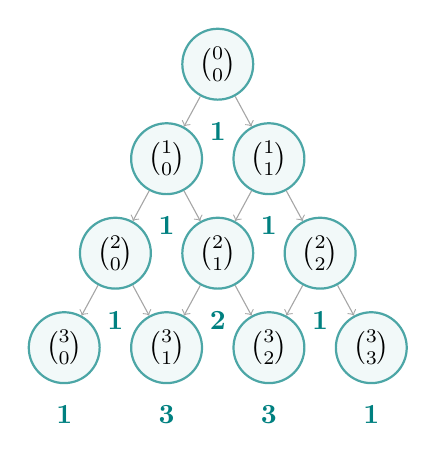
\begin{tikzpicture}[x=1.3cm,y=1.0cm,
  row/.style={draw=none,fill=none},
  node/.style={circle,draw=teal!70,fill=teal!5,thick,minimum size=9mm,inner sep=0pt}]
  
  % Row 0
  \node[node] (n0k0) at (0,0) {$\binom{0}{0}$};
  \node[below=1.5mm of n0k0,teal] {\textbf{1}};
  
  % Row 1
  \node[node] (n1k0) at (-0.5,-1.2) {$\binom{1}{0}$};
  \node[below=1.5mm of n1k0,teal] {\textbf{1}};
  \node[node] (n1k1) at (0.5,-1.2) {$\binom{1}{1}$};
  \node[below=1.5mm of n1k1,teal] {\textbf{1}};
  
  % Row 2
  \node[node] (n2k0) at (-1.0,-2.4) {$\binom{2}{0}$};
  \node[below=1.5mm of n2k0,teal] {\textbf{1}};
  \node[node] (n2k1) at (0,-2.4) {$\binom{2}{1}$};
  \node[below=1.5mm of n2k1,teal] {\textbf{2}};
  \node[node] (n2k2) at (1.0,-2.4) {$\binom{2}{2}$};
  \node[below=1.5mm of n2k2,teal] {\textbf{1}};
  
  % Row 3
  \node[node] (n3k0) at (-1.5,-3.6) {$\binom{3}{0}$};
  \node[below=1.5mm of n3k0,teal] {\textbf{1}};
  \node[node] (n3k1) at (-0.5,-3.6) {$\binom{3}{1}$};
  \node[below=1.5mm of n3k1,teal] {\textbf{3}};
  \node[node] (n3k2) at (0.5,-3.6) {$\binom{3}{2}$};
  \node[below=1.5mm of n3k2,teal] {\textbf{3}};
  \node[node] (n3k3) at (1.5,-3.6) {$\binom{3}{3}$};
  \node[below=1.5mm of n3k3,teal] {\textbf{1}};
  
  % Connections showing Pascal's Identity
  \draw[->,thin,gray!70] (n0k0) -- (n1k0);
  \draw[->,thin,gray!70] (n0k0) -- (n1k1);
  \draw[->,thin,gray!70] (n1k0) -- (n2k0);
  \draw[->,thin,gray!70] (n1k0) -- (n2k1);
  \draw[->,thin,gray!70] (n1k1) -- (n2k1);
  \draw[->,thin,gray!70] (n1k1) -- (n2k2);
  \draw[->,thin,gray!70] (n2k0) -- (n3k0);
  \draw[->,thin,gray!70] (n2k0) -- (n3k1);
  \draw[->,thin,gray!70] (n2k1) -- (n3k1);
  \draw[->,thin,gray!70] (n2k1) -- (n3k2);
  \draw[->,thin,gray!70] (n2k2) -- (n3k2);
  \draw[->,thin,gray!70] (n2k2) -- (n3k3);
\end{tikzpicture}
\end{center}

\subsection{Key Invariants and Properties}

Pascal's Triangle exhibits several core mathematical invariants:
\begin{enumerate}
    \item \textbf{Symmetry:} Within any row $n$, the coefficients are symmetric about the center:
    \begin{equation}
    \binom{n}{k} = \binom{n}{n - k}
    \end{equation}
    \item \textbf{Sum of Row Elements:} The sum of all elements in row $n$ is $2^n$:
    \begin{equation}
    \sum_{k=0}^{n} \binom{n}{k} = 2^n
    \end{equation}
    \item \textbf{Alternating Row Sum:} The alternating sum of elements in row $n$ is $0$ (for $n \ge 1$):
    \begin{equation}
    \sum_{k=0}^{n} (-1)^k \binom{n}{k} = 0
    \end{equation}
    \item \textbf{Hockey Stick Identity:} The sum of consecutive binomial coefficients starting from the boundary equals a single coefficient in the next row:
    \begin{equation}
    \sum_{i=r}^{n} \binom{i}{r} = \binom{n+1}{r+1}
    \end{equation}
\end{enumerate}

\subsection{Algorithmic Construction Paradigms}

To construct the first $N$ rows of Pascal's Triangle, we analyze three different algorithmic approaches and contrast their performance.

\subsubsection{Approach 1: Naive Recursive Formulation}

Based directly on Pascal's Identity, we can implement a recursive method to fetch any coefficient $\binom{n}{k}$:
\begin{equation}
f(n, k) = f(n-1, k-1) + f(n-1, k)
\end{equation}
Computing an entire row $N$ using this method incurs severe overlapping subproblems. The recursive call tree for $\binom{N}{K}$ matches the structure of the Fibonacci recursion, leading to an exponential time complexity:
\begin{equation}
T_{\text{naive}}(N) = \mathcal{O}(2^N)
\end{equation}
The space complexity is determined by the maximum depth of the call stack, which is $\mathcal{O}(N)$.

\subsubsection{Approach 2: Standard 2D Dynamic Programming}

We can avoid recomputing subproblems by storing previously computed coefficients in a 2D grid structure. This is a classic application of dynamic programming.

\begin{verbatim}
import java.util.ArrayList;
import java.util.List;

public class PascalsTriangle2DDP {
    public static List<List<Integer>> generate(int numRows) {
        List<List<Integer>> triangle = new ArrayList<>();
        if (numRows <= 0) return triangle;

        // Initialize row 0
        List<Integer> firstRow = new ArrayList<>();
        firstRow.add(1);
        triangle.add(firstRow);

        for (int i = 1; i < numRows; i++) {
            List<Integer> row = new ArrayList<>();
            List<Integer> prevRow = triangle.get(i - 1);

            row.add(1); // Boundary element
            for (int j = 1; j < i; j++) {
                // Apply Pascal's Identity
                row.add(prevRow.get(j - 1) + prevRow.get(j));
            }
            row.add(1); // Boundary element
            triangle.add(row);
        }
        return triangle;
    }
}
\end{verbatim}

\begin{itemize}
    \item \textbf{Time Complexity:} We execute a nested loop where the outer loop runs $N$ times and the inner loop runs up to $i$ times. The total number of additions is:
    \begin{equation}
    \sum_{i=1}^{N-1} (i - 1) = \frac{(N-1)(N-2)}{2} = \mathcal{O}(N^2)
    \end{equation}
    \item \textbf{Space Complexity:} To store the output, we occupy memory proportional to the size of the triangle:
    \begin{equation}
    S(N) = \sum_{i=1}^{N} i = \frac{N(N+1)}{2} = \mathcal{O}(N^2)
    \end{equation}
\end{itemize}

\subsubsection{Approach 3: Space-Optimized 1D Dynamic Programming}

If the goal is to generate only a specific row $N$ of Pascal's Triangle rather than the entire history, we do not need to persist a 2D table. We can update a single 1D array in-place. To prevent overwriting values before they are used in the calculation, we must iterate backwards (from right to left).

\begin{verbatim}
import java.util.ArrayList;
import java.util.List;

public class PascalsTriangle1DDP {
    public static List<Integer> getRow(int rowIndex) {
        List<Integer> row = new ArrayList<>(rowIndex + 1);
        // Initialize all elements to 0, except the first which is 1
        row.add(1);
        for (int i = 1; i <= rowIndex; i++) {
            row.add(0);
        }

        for (int i = 1; i <= rowIndex; i++) {
            for (int j = i; j >= 1; j--) {
                row.set(j, row.get(j) + row.get(j - 1));
            }
        }
        return row;
    }
}
\end{verbatim}

\begin{itemize}
    \item \textbf{Time Complexity:} Still requires computing the sum of elements, leading to $\mathcal{O}(N^2)$ iterations.
    \item \textbf{Space Complexity:} Only the 1D state is maintained in memory. Thus:
    \begin{equation}
    S_{\text{opt}}(N) = \mathcal{O}(N) \quad \text{(excluding the return list space)}
    \end{equation}
\end{itemize}

%% ============================================================
\section{The Binomial Theorem and Mathematical Proofs}
\label{sec:binomial}

The Binomial Theorem provides a closed-form algebraic expansion for the powers of a binomial expression.

\subsection{Theorem Statement}

\begin{theorem}[The Binomial Theorem]
For any real (or complex) variables $x$ and $y$, and any non-negative integer $n$:
\begin{equation}
(x + y)^n = \sum_{k=0}^{n} \binom{n}{k} x^{n - k} y^k
\end{equation}
\end{theorem}

The general term in the expansion, representing the $(k+1)$-th term, is formulated as:
\begin{equation}
T_{k+1} = \binom{n}{k} x^{n - k} y^k
\end{equation}

\subsection{Inductive Proof}

We prove the Binomial Theorem using the Principle of Mathematical Induction on the variable $n$.

\begin{proof}
\textbf{Base Case ($n = 0$):}
\begin{equation}
(x + y)^0 = 1 \quad \text{and} \quad \sum_{k=0}^{0} \binom{0}{k} x^{0-k} y^k = \binom{0}{0} x^0 y^0 = 1
\end{equation}
The base case holds.

\textbf{Inductive Hypothesis:}
Assume the theorem is true for some positive integer $m \ge 0$:
\begin{equation}
(x + y)^m = \sum_{k=0}^{m} \binom{m}{k} x^{m - k} y^k
\end{equation}

\textbf{Inductive Step:}
We show that the theorem holds for $n = m + 1$:
\begin{equation}
(x + y)^{m+1} = (x + y) (x + y)^m
\end{equation}
Substituting the induction hypothesis:
\begin{align}
(x + y)^{m+1} &= (x + y) \sum_{k=0}^{m} \binom{m}{k} x^{m - k} y^k \\
&= x \sum_{k=0}^{m} \binom{m}{k} x^{m - k} y^k + y \sum_{k=0}^{m} \binom{m}{k} x^{m - k} y^k \\
&= \sum_{k=0}^{m} \binom{m}{k} x^{m - k + 1} y^k + \sum_{k=0}^{m} \binom{m}{k} x^{m - k} y^{k + 1}
\end{align}
For the first sum, we isolate the term for $k = 0$:
\begin{equation}
\sum_{k=0}^{m} \binom{m}{k} x^{m - k + 1} y^k = \binom{m}{0} x^{m+1} y^0 + \sum_{k=1}^{m} \binom{m}{k} x^{m - k + 1} y^k
\end{equation}
For the second sum, we make a change of variable by letting $j = k + 1$ (hence $k = j - 1$):
\begin{equation}
\sum_{k=0}^{m} \binom{m}{k} x^{m - k} y^{k+1} = \sum_{j=1}^{m+1} \binom{m}{j - 1} x^{m - (j - 1)} y^j = \sum_{j=1}^{m} \binom{m}{j - 1} x^{m - j + 1} y^j + \binom{m}{m} x^0 y^{m+1}
\end{equation}
Since $j$ is a dummy variable of summation, we can replace it with $k$:
\begin{equation}
= \sum_{k=1}^{m} \binom{m}{k - 1} x^{m - k + 1} y^k + \binom{m}{m} y^{m+1}
\end{equation}
Substituting these two decomposed expansions back:
\begin{align}
(x + y)^{m+1} &= \binom{m}{0} x^{m+1} + \sum_{k=1}^{m} \binom{m}{k} x^{m - k + 1} y^k + \sum_{k=1}^{m} \binom{m}{k - 1} x^{m - k + 1} y^k + \binom{m}{m} y^{m+1} \\
&= \binom{m}{0} x^{m+1} + \sum_{k=1}^{m} \left[ \binom{m}{k} + \binom{m}{k - 1} \right] x^{m - k + 1} y^k + \binom{m}{m} y^{m+1}
\end{align}
Applying Pascal's Identity $\binom{m}{k} + \binom{m}{k - 1} = \binom{m+1}{k}$:
\begin{equation}
(x + y)^{m+1} = \binom{m}{0} x^{m+1} + \sum_{k=1}^{m} \binom{m+1}{k} x^{m+1 - k} y^k + \binom{m}{m} y^{m+1}
\end{equation}
Note that $\binom{m}{0} = 1 = \binom{m+1}{0}$ and $\binom{m}{m} = 1 = \binom{m+1}{m+1}$. We can integrate the boundary terms into the summation:
\begin{align}
(x + y)^{m+1} &= \binom{m+1}{0} x^{m+1 - 0} y^0 + \sum_{k=1}^{m} \binom{m+1}{k} x^{m+1 - k} y^k + \binom{m+1}{m+1} x^0 y^{m+1} \\
&= \sum_{k=0}^{m+1} \binom{m+1}{k} x^{m+1 - k} y^k
\end{align}
The formula holds for $n = m+1$. By the Principle of Mathematical Induction, the Binomial Theorem is true for all integers $n \geq 0$.
\end{proof}

\subsection{Combinatorial Proof}

Consider the product:
\begin{equation}
(x + y)^n = \underbrace{(x + y)(x + y) \cdots (x + y)}_{n \text{ factors}}
\end{equation}
When expanding this product, we form terms by choosing either $x$ or $y$ from each of the $n$ factors. A term of the form $x^{n-k}y^k$ arises when we choose $y$ from exactly $k$ factors and $x$ from the remaining $n-k$ factors. 

The number of ways to choose $k$ factors from a set of $n$ factors is given by the combination $\binom{n}{k}$. Thus, the coefficient of $x^{n-k}y^k$ in the expanded expression is exactly $\binom{n}{k}$. Summing over all possible values of $k$ from $0$ to $n$ yields:
\begin{equation}
(x + y)^n = \sum_{k=0}^{n} \binom{n}{k} x^{n - k} y^k
\end{equation}

\subsection{Middle Terms in Binomial Expansion}

Locating the middle term(s) of $(x+y)^n$ depends on the parity of $n$:
\begin{itemize}
    \item \textbf{Case 1: $n$ is even.} The expansion contains $n+1$ terms (an odd number). There is a single middle term, which is the $(\frac{n}{2} + 1)$-th term:
    \begin{equation}
    T_{\text{mid}} = T_{\frac{n}{2} + 1} = \binom{n}{n/2} x^{n/2} y^{n/2}
    \end{equation}
    \item \textbf{Case 2: $n$ is odd.} The expansion contains $n+1$ terms (an even number). There are two middle terms, namely the $(\frac{n+1}{2})$-th and $(\frac{n+3}{2})$-th terms:
    \begin{equation}
    T_{\text{mid}, 1} = T_{\frac{n+1}{2}} = \binom{n}{\frac{n-1}{2}} x^{\frac{n+1}{2}} y^{\frac{n-1}{2}}
    \end{equation}
    \begin{equation}
    T_{\text{mid}, 2} = T_{\frac{n+3}{2}} = \binom{n}{\frac{n+1}{2}} x^{\frac{n-1}{2}} y^{\frac{n+1}{2}}
    \end{equation}
\end{itemize}

\subsection{Constant Terms (Terms Independent of $x$)}

In algebraic expressions of the form $(ax^p + \frac{b}{x^q})^n$, we are often tasked with finding the term that does not contain $x$ (the constant term). We locate this by writing the general term:
\begin{equation}
T_{k+1} = \binom{n}{k} (ax^p)^{n-k} \left(\frac{b}{x^q}\right)^k = \binom{n}{k} a^{n-k} b^k x^{p(n-k) - qk}
\end{equation}
To make this term independent of $x$, we set the exponent of $x$ to $0$:
\begin{equation}
p(n-k) - qk = 0 \implies pn - (p+q)k = 0 \implies k = \frac{pn}{p+q}
\end{equation}
If $k$ is a non-negative integer such that $0 \le k \le n$, the constant term exists and is given by $T_{k+1}$. Otherwise, no constant term exists.

\subsection{Rational and Irrational Terms}

In expansions of the form $(a^{1/p} + b^{1/q})^n$, where $a, b$ are distinct prime numbers, the terms are rational if and only if the exponents of both terms are integers. The general term is:
\begin{equation}
T_{k+1} = \binom{n}{k} (a^{1/p})^{n-k} (b^{1/q})^k = \binom{n}{k} a^{\frac{n-k}{p}} b^{\frac{k}{q}}
\end{equation}
For $T_{k+1}$ to be rational, we require:
\begin{equation}
\frac{n-k}{p} \in \mathbb{Z} \quad \text{and} \quad \frac{k}{q} \in \mathbb{Z} \quad \text{for } 0 \le k \le n
\end{equation}
This means $k$ must be a multiple of $q$, and $n-k$ must be a multiple of $p$. Finding the number of rational terms amounts to finding the number of integer values of $k$ that satisfy these simultaneous divisibility constraints. The remaining terms in the expansion ($n + 1 - N_{\text{rational}}$) are irrational.

\subsection{Vandermonde's Identity (Sum of Squares of Coefficients)}

Vandermonde's Identity provides a beautiful formulation for the sum of the squares of the binomial coefficients.

\begin{theorem}[Vandermonde's Identity for Squares]
For any positive integer $n$:
\begin{equation}
\sum_{k=0}^{n} \binom{n}{k}^2 = \binom{2n}{n}
\end{equation}
\end{theorem}

\begin{proof}
Consider the identity:
\begin{equation}
(1+x)^{2n} = (1+x)^n (1+x)^n
\end{equation}
Using the Binomial Theorem, the coefficient of $x^n$ on the left-hand side of the equation is:
Using the Binomial Theorem, the coefficient of $x^n$ on the left-hand side of the equation is:
\begin{equation}
\text{Coeff of } x^n \text{ in } (1+x)^{2n} = \binom{2n}{n}
\end{equation}
On the right-hand side, we expand both factors:
\begin{equation}
(1+x)^n (1+x)^n = \left( \sum_{i=0}^{n} \binom{n}{i} x^i \right) \left( \sum_{j=0}^{n} \binom{n}{j} x^j \right)
\end{equation}
To obtain a term of degree $n$ in the product, we must multiply a term of degree $i$ from the first factor by a term of degree $n-i$ from the second factor. The coefficient of $x^n$ is the sum of these products over all valid $i$:
\begin{equation}
\text{Coeff of } x^n = \sum_{i=0}^{n} \binom{n}{i} \binom{n}{n-i}
\end{equation}
By the symmetry property of binomial coefficients, we know that $\binom{n}{n-i} = \binom{n}{i}$. Substituting this in yields:
\begin{equation}
\text{Coeff of } x^n = \sum_{i=0}^{n} \binom{n}{i} \binom{n}{i} = \sum_{i=0}^{n} \binom{n}{i}^2
\end{equation}
Equating the coefficients of $x^n$ from both sides:
\begin{equation}
\sum_{k=0}^{n} \binom{n}{k}^2 = \binom{2n}{n}
\end{equation}
This completes the proof.
\end{proof}

\subsection{Numerically Greatest Term (NGT)}

For a given real value of $x$, the terms in the expansion of $(1+x)^n$ vary in magnitude. We want to find the index $r$ that yields the numerically greatest term, $T_{r+1}$.

We define $T_{r+1}$ to be the numerically greatest term if:
\begin{equation}
|T_{r+1}| \ge |T_r| \quad \text{and} \quad |T_{r+1}| \ge |T_{r+2}|
\end{equation}
To find this index, we examine the ratio of consecutive terms in $(1+x)^n$:
\begin{equation}
\frac{|T_{r+1}|}{|T_r|} = \frac{\left| \binom{n}{r} x^r \right|}{\left| \binom{n}{r-1} x^{r-1} \right|} = \frac{n-r+1}{r} |x|
\end{equation}
Setting this ratio to be greater than or equal to $1$:
\begin{align}
\frac{n-r+1}{r} |x| \ge 1 &\implies (n-r+1)|x| \ge r \\
& \implies (n+1)|x| - r|x| \ge r \\
& \implies (n+1)|x| \ge r(1 + |x|) \\
& \implies r \le \frac{(n+1)|x|}{1 + |x|}
\end{align}
Let:
\begin{equation}
m = \frac{(n+1)|x|}{1 + |x|}
\end{equation}
\begin{enumerate}
    \item \textbf{Case 1: $m$ is an integer.} In this case, the ratio equals $1$ when $r = m$. This means $|T_{m+1}| = |T_m|$, and both terms are numerically greatest.
    \item \textbf{Case 2: $m$ is not an integer.} The largest integer $r$ satisfying the inequality is $r = \lfloor m \rfloor$. The single numerically greatest term is $T_{\lfloor m \rfloor + 1}$.
\end{enumerate}

\subsection{Important Corollaries and Algebraic Identities}

By substituting specific values for $x$ and $y$, we derive standard identities frequently tested in competitive examinations.

\begin{corollary}[Sum of Coefficients]
Let $x = 1, y = 1$:
\begin{equation}
(1 + 1)^n = \sum_{k=0}^{n} \binom{n}{k} 1^{n-k} 1^k \implies \sum_{k=0}^{n} \binom{n}{k} = 2^n
\end{equation}
This shows that the sum of binomial coefficients of order $n$ is $2^n$.
\end{corollary}

\begin{corollary}[Alternating Sum of Coefficients]
Let $x = 1, y = -1$:
\begin{equation}
(1 - 1)^n = \sum_{k=0}^{n} \binom{n}{k} 1^{n-k} (-1)^k \implies \sum_{k=0}^{n} (-1)^k \binom{n}{k} = 0 \quad \text{for } n \ge 1
\end{equation}
Equivalently:
\begin{equation}
\binom{n}{0} + \binom{n}{2} + \binom{n}{4} + \cdots = \binom{n}{1} + \binom{n}{3} + \binom{n}{5} + \cdots = 2^{n-1}
\end{equation}
The sum of even-indexed coefficients equals the sum of odd-indexed coefficients, both equal to $2^{n-1}$.
\end{corollary}

\begin{corollary}[Derivative-based Identity]
Consider the binomial expansion of $(1 + x)^n$:
\begin{equation}
(1 + x)^n = \sum_{k=0}^{n} \binom{n}{k} x^k
\end{equation}
Differentiating both sides with respect to $x$:
\begin{equation}
n(1 + x)^{n-1} = \sum_{k=1}^{n} k \binom{n}{k} x^{k-1}
\end{equation}
Substituting $x = 1$:
\begin{equation}
\sum_{k=1}^{n} k \binom{n}{k} = n \cdot 2^{n-1}
\end{equation}
\end{corollary}

\begin{corollary}[Integration-based Identity]
Consider the integration of $(1+x)^n$ from $0$ to $1$:
\begin{equation}
\int_{0}^{1} (1+x)^n dx = \int_{0}^{1} \left( \sum_{k=0}^{n} \binom{n}{k} x^k \right) dx
\end{equation}
Evaluating the integrals:
\begin{equation}
\left[ \frac{(1+x)^{n+1}}{n+1} \right]_{0}^{1} = \sum_{k=0}^{n} \binom{n}{k} \left[ \frac{x^{k+1}}{k+1} \right]_{0}^{1}
\end{equation}
\begin{equation}
\frac{2^{n+1} - 1}{n+1} = \sum_{k=0}^{n} \frac{1}{k+1} \binom{n}{k}
\end{equation}
\end{corollary}

%% ============================================================
\section{The Multinomial Theorem and Multiset Permutations}
\label{sec:multinomial}

The Multinomial Theorem generalizes the Binomial Theorem to expansions of polynomials with $m$ terms.

\subsection{Theorem Statement}

\begin{theorem}[The Multinomial Theorem]
For any positive integer $n$ and any real variables $x_1, x_2, \ldots, x_m$:
\begin{equation}
(x_1 + x_2 + \cdots + x_m)^n = \sum_{k_1+k_2+\cdots+k_m=n} \binom{n}{k_1, k_2, \ldots, k_m} \prod_{i=1}^{m} x_i^{k_i}
\end{equation}
where the summation is taken over all non-negative integer sequences $(k_1, k_2, \ldots, k_m)$ such that $k_1 + k_2 + \cdots + k_m = n$.
\end{theorem}

The multinomial coefficient is defined as:
\begin{equation}
\binom{n}{k_1, k_2, \ldots, k_m} = \frac{n!}{k_1! k_2! \cdots k_m!}
\end{equation}

\subsection{Derivation via Multiset Permutations}

Consider a multiset containing $n$ total objects, where there are $m$ distinct types of objects, and the count of objects of type $i$ is $k_i$ (so that $\sum_{i=1}^{m} k_i = n$). The number of distinct linear permutations of this multiset is given by the multinomial coefficient.

\begin{proof}
We want to arrange $n$ items in $n$ sequential slots. 
\begin{enumerate}
    \item We choose $k_1$ slots out of $n$ for the objects of type 1. This can be done in $\binom{n}{k_1}$ ways.
    \item Out of the remaining $n - k_1$ slots, we choose $k_2$ slots for the objects of type 2. This can be done in $\binom{n - k_1}{k_2}$ ways.
    \item Similarly, for the $i$-th type, we choose $k_i$ slots from the remaining $n - \sum_{j=1}^{i-1} k_j$ slots in $\binom{n - \sum_{j=1}^{i-1} k_j}{k_i}$ ways.
\end{enumerate}
By the product rule, the total number of permutations is the product of these selections:
\begin{align}
\text{Total Permutations} &= \binom{n}{k_1} \binom{n - k_1}{k_2} \binom{n - k_1 - k_2}{k_3} \cdots \binom{n - k_1 - \cdots - k_{m-1}}{k_m} \\
&= \frac{n!}{k_1!(n-k_1)!} \cdot \frac{(n-k_1)!}{k_2!(n-k_1-k_2)!} \cdot \frac{(n-k_1-k_2)!}{k_3!(n-k_1-k_2-k_3)!} \cdots \frac{(n-k_1-\cdots-k_{m-1})!}{k_m!(0)!}
\end{align}
Observe the telescoping cancellations of terms in the numerators and denominators:
\begin{equation}
= \frac{n!}{k_1! k_2! k_3! \cdots k_m!} = \binom{n}{k_1, k_2, \ldots, k_m}
\end{equation}
This completes the derivation.
\end{proof}

\subsection{Sum of Multinomial Coefficients}

The sum of all multinomial coefficients for a given $n$ and $m$ can be found by evaluating the expansion where all variables are set to $1$. 

\begin{theorem}[Sum of Multinomial Coefficients]
The sum of all multinomial coefficients for parameters $n$ and $m$ is:
\begin{equation}
\sum_{k_1+k_2+\cdots+k_m=n} \binom{n}{k_1, k_2, \ldots, k_m} = m^n
\end{equation}
\end{theorem}

\begin{proof}
Let $x_1 = x_2 = \cdots = x_m = 1$ in the Multinomial Theorem:
\begin{align}
(1 + 1 + \cdots + 1)^n &= \sum_{k_1+k_2+\cdots+k_m=n} \binom{n}{k_1, k_2, \ldots, k_m} (1)^{k_1} (1)^{k_2} \cdots (1)^{k_m} \\
m^n &= \sum_{k_1+k_2+\cdots+k_m=n} \binom{n}{k_1, k_2, \ldots, k_m}
\end{align}
This proves the sum of all coefficients equals $m^n$.
\end{proof}

\subsection{Number of Terms in a Multinomial Expansion}

A common question in combinatorial exams is finding the total number of distinct terms in the expanded form of a multinomial.

\begin{theorem}[Number of Terms]
The number of distinct terms in the expansion of $(x_1 + x_2 + \cdots + x_m)^n$ is:
\begin{equation}
N_{\text{terms}} = \binom{n + m - 1}{m - 1}
\end{equation}
\end{theorem}

\begin{proof}
Each term in the expansion is uniquely determined by the exponents $(k_1, k_2, \ldots, k_m)$ of the product $x_1^{k_1} x_2^{k_2} \cdots x_m^{k_m}$. Since these exponents must be non-negative integers satisfying:
\begin{equation}
k_1 + k_2 + \cdots + k_m = n \quad \text{where } k_i \ge 0
\end{equation}
the number of distinct terms corresponds exactly to the number of non-negative integer solutions to this linear Diophantine equation.

We model this using the classic "Stars and Bars" combinatorial method. Let there be $n$ identical stars representing the total degree, and $m - 1$ bars acting as dividers separating the variables. The number of ways to arrange $n$ stars and $m - 1$ bars in a linear sequence is:
\begin{equation}
\binom{\text{stars} + \text{bars}}{\text{bars}} = \binom{n + (m - 1)}{m - 1} = \binom{n + m - 1}{m - 1}
\end{equation}
This proves the theorem.
\end{proof}

%% ============================================================
\section{Modular Combinatorics in Competitive Programming}
\label{sec:modular}

In competitive programming, calculations are almost always performed modulo a large prime, typically $P = 10^9+7$ or $P = 998244353$. This is to prevent integer overflow and focus on algebraic logic.

\subsection{Fermat's Little Theorem and Modular Division}

Since division is not directly compatible with modular arithmetic, we compute the modular multiplicative inverse of a denominator.

\begin{theorem}[Fermat's Little Theorem]
If $P$ is a prime number and $a$ is an integer not divisible by $P$, then:
\begin{equation}
a^{P-1} \equiv 1 \pmod P
\end{equation}
Multiplying both sides by $a^{-1}$ gives the modular multiplicative inverse:
\begin{equation}
a^{-2} \equiv a^{-1} \pmod P \implies a^{-1} \equiv a^{P-2} \pmod P
\end{equation}
\end{theorem}
This allows us to evaluate modular division $\frac{A}{B} \pmod P$ as:
\begin{equation}
A \cdot B^{-1} \equiv A \cdot B^{P-2} \pmod P
\end{equation}

\subsection{Linear Precomputation of Combination Queries}

To answer queries of $\binom{N}{K} \pmod P$ in $\mathcal{O}(1)$ time, we precompute factorials and inverse factorials up to the maximum capacity $MAX\_N$.

\begin{verbatim}
public class ModularCombinatorics {
    private static final int MOD = 1_000_000_007;
    private static long[] fact;
    private static long[] invFact;

    public static void precompute(int maxN) {
        fact = new long[maxN + 1];
        invFact = new long[maxN + 1];
        
        fact[0] = 1;
        for (int i = 1; i <= maxN; i++) {
            fact[i] = (fact[i - 1] * i) % MOD;
        }

        // Compute invFact[maxN] using binary exponentiation: fact[maxN]^(MOD-2)
        invFact[maxN] = power(fact[maxN], MOD - 2);

        // Linear backward scan for inverse factorials
        for (int i = maxN - 1; i >= 0; i--) {
            invFact[i] = (invFact[i + 1] * (i + 1)) % MOD;
        }
    }

    public static long nCr(int n, int r) {
        if (r < 0 || r > n) return 0;
        return fact[n] * invFact[r] % MOD * invFact[n - r] % MOD;
    }

    private static long power(long base, long exp) {
        long res = 1;
        base %= MOD;
        while (exp > 0) {
            if ((exp & 1) == 1) res = (res * base) % MOD;
            base = (base * base) % MOD;
            exp >>= 1;
        }
        return res;
    }
}
\end{verbatim}

\begin{itemize}
    \item \textbf{Preprocessing Time Complexity:} $\mathcal{O}(N)$ for factorial loops and $\mathcal{O}(\log P)$ for the boundary exponentiation.
    \item \textbf{Query Time Complexity:} $\mathcal{O}(1)$ multiplications.
    \item \textbf{Space Complexity:} $\mathcal{O}(N)$ memory allocations.
\end{itemize}

%% ============================================================
\section{Advanced Counting Sequences: Catalan Numbers and Derangements}
\label{sec:sequences}

Beyond direct selection counts, two advanced combinatorial sequences appear constantly in algorithm analysis.

\subsection{Catalan Numbers}

\begin{definition}[Catalan Number]
The $n$-th Catalan number $C_n$ represents the number of valid configurations of various recursive structures. The explicit formula in terms of binomial coefficients is:
\begin{equation}
C_n = \frac{1}{n+1} \binom{2n}{n} = \binom{2n}{n} - \binom{2n}{n-1}
\end{equation}
\end{definition}

The sequence satisfies the fundamental recurrence relation:
\begin{equation}
C_0 = 1, \quad C_{n+1} = \sum_{i=0}^{n} C_i C_{n-i}
\end{equation}

\subsubsection{Key Applications}
\begin{enumerate}
    \item \textbf{Dyck Paths:} Number of paths on a grid from $(0,0)$ to $(2n, 0)$ moving only diagonal-up and diagonal-down that never dip below the x-axis.
    \item \textbf{Balanced Parentheses:} Number of unique strings containing exactly $n$ left brackets and $n$ right brackets that are legally balanced (e.g., LeetCode "Generate Parentheses").
    \item \textbf{Binary Search Trees:} Number of distinct binary search trees that can be formed using $n$ unique keys (e.g., LeetCode "Unique Binary Search Trees").
\end{enumerate}

\subsection{Derangements}

\begin{definition}[Derangement]
A \emph{derangement} is a permutation of a set of $n$ elements in which no element appears in its original position. The number of derangements is denoted by $D_n$ or $!n$.
\end{definition}

\subsubsection{Recurrence Relations and Closed Form}
Using the Principle of Inclusion-Exclusion (PIE), we derive the closed form:
\begin{equation}
D_n = n! \sum_{i=0}^{n} \frac{(-1)^i}{i!} = n! \left( 1 - \frac{1}{1!} + \frac{1}{2!} - \frac{1}{3!} + \cdots + \frac{(-1)^n}{n!} \right)
\end{equation}
It can be computed dynamically using the simple recurrences:
\begin{equation}
D_n = (n-1)(D_{n-1} + D_{n-2}) \quad \text{for } n \ge 2
\end{equation}
\begin{equation}
D_n = n D_{n-1} + (-1)^n \quad \text{for } n \ge 1
\end{equation}
with base cases $D_0 = 1, D_1 = 0$.

%% ============================================================
\section{Lucas' Theorem for Large Combinations}
\label{sec:lucas}

When we need to evaluate $\binom{N}{K} \pmod P$ under huge constraints ($N, K \le 10^{18}$) but the prime modulo $P$ is relatively small ($P < 10^6$), standard factorial precomputation fails because $N \ge P$ yields factorials congruent to $0 \pmod P$. To bypass this, we use Lucas' Theorem.

\begin{theorem}[Lucas' Theorem]
For non-negative integers $N$ and $K$ and a prime $P$, write the base-$P$ expansions of $N$ and $K$:
\begin{align}
N &= n_s P^s + n_{s-1} P^{s-1} + \cdots + n_1 P + n_0 \\
K &= k_s P^s + k_{s-1} P^{s-1} + \cdots + k_1 P + k_0
\end{align}
where $0 \le n_i, k_i < P$. Then:
\begin{equation}
\binom{N}{K} \equiv \prod_{i=0}^{s} \binom{n_i}{k_i} \pmod P
\end{equation}
where $\binom{n_i}{k_i} = 0$ if $n_i < k_i$.
\end{theorem}

\subsection{Algorithmic Implementation}
The calculation repeatedly extracts the remainder modulo $P$ (the digits) and multiplies the sub-combinations.

\begin{verbatim}
public class LucasCombination {
    private static int P;

    // Standard nCr modulo P for small inputs (n, r < P)
    private static long smallNCr(int n, int r, long[] fact, long[] invFact) {
        if (r < 0 || r > n) return 0;
        return fact[n] * invFact[r] % P * invFact[n - r] % P;
    }

    public static long lucasNCr(long n, long r, long[] fact, long[] invFact) {
        if (r == 0) return 1;
        int ni = (int) (n % P);
        int ki = (int) (r % P);
        return (lucasNCr(n / P, r / P, fact, invFact) * smallNCr(ni, ki, fact, invFact)) % P;
    }
}
\end{verbatim}

\begin{itemize}
    \item \textbf{Time Complexity:} The division loops $s = \mathcal{O}(\log_P N)$ times. Thus, the computation runs in logarithmic time.
    \item \textbf{Space Complexity:} $\mathcal{O}(P)$ for factorial precomputation of the base values.
\end{itemize}

%% ============================================================
\section{Stirling Numbers and Set Partitions}
\label{sec:stirling}

In discrete mathematics, partitioning distinct items into equivalent clusters requires a different set of coefficients.

\begin{definition}[Stirling Numbers of the Second Kind]
The Stirling number of the second kind, denoted by $S(n, k)$ or $\left\{ \begin{matrix} n \\ k \end{matrix} \right\}$, represents the number of ways to partition a set of $n$ labeled elements into $k$ unlabeled, non-empty subsets.
\end{definition}

\subsection{Recurrence Relation}
The Stirling numbers satisfy the recurrence:
\begin{equation}
S(n, k) = k \cdot S(n - 1, k) + S(n - 1, k - 1) \quad \text{for } 1 \le k \le n
\end{equation}
with base cases:
\begin{align}
S(0, 0) &= 1 \\
S(n, 0) &= 0 \quad \text{for } n > 0 \\
S(n, k) &= 0 \quad \text{for } k > n
\end{align}

\subsection{Combinatorial Proof of Recurrence}
Consider a specific target element $x \in S$, where $|S| = n$. When partitioning $S$ into $k$ subsets:
\begin{enumerate}
    \item \textbf{Case 1:} Element $x$ is placed in its own singleton subset $\{x\}$. The remaining $n-1$ elements must be partitioned into $k-1$ subsets. The count of such partitions is $S(n - 1, k - 1)$.
    \item \textbf{Case 2:} Element $x$ is placed in a subset containing other elements. The remaining $n-1$ elements are partitioned into $k$ subsets first. Then, element $x$ can be inserted into any of these $k$ subsets. The count of such arrangements is $k \cdot S(n - 1, k)$.
\end{enumerate}
Summing these two mutually exclusive cases yields the recurrence relation.

\subsection{Dynamic Programming Implementation}
Stirling numbers can be precomputed using a 2D dynamic programming grid.

\begin{verbatim}
public class StirlingNumbers {
    public static long[][] computeStirling(int n, int k) {
        long[][] dp = new long[n + 1][k + 1];
        dp[0][0] = 1;

        for (int i = 1; i <= n; i++) {
            for (int j = 1; j <= Math.min(i, k); j++) {
                dp[i][j] = (j * dp[i - 1][j] + dp[i - 1][j - 1]);
            }
        }
        return dp;
    }
}
\end{verbatim}
The time and space complexities are both $\mathcal{O}(N \cdot K)$.

%% ============================================================
\section{The Inclusion-Exclusion Principle (PIE)}
\label{sec:pie}

The Principle of Inclusion-Exclusion (PIE) is a general counting technique used to find the cardinality of the union of multiple finite sets.

\begin{theorem}[Principle of Inclusion-Exclusion]
Let $A_1, A_2, \ldots, A_m$ be finite sets. Then:
\begin{equation}
\left| \bigcup_{i=1}^{m} A_i \right| = \sum_{i=1}^{m} |A_i| - \sum_{1 \le i < j \le m} |A_i \cap A_j| + \sum_{1 \le i < j < k \le m} |A_i \cap A_j \cap A_k| - \cdots + (-1)^{m-1} |A_1 \cap A_2 \cap \cdots \cap A_m|
\end{equation}
\end{theorem}

In compact notation:
\begin{equation}
\left| \bigcup_{i=1}^{m} A_i \right| = \sum_{\emptyset \neq J \subseteq \{1, \ldots, m\}} (-1)^{|J|-1} \left| \bigcap_{j \in J} A_j \right|
\end{equation}

We can find the cardinality of the complement (elements belonging to none of the sets) using:
\begin{equation}
\left| \bigcap_{i=1}^{m} A_i^c \right| = |U| - \left| \bigcup_{i=1}^{m} A_i \right|
\end{equation}
where $U$ is the universal set.

%% ============================================================
\section{The Pigeonhole Principle (PHP)}
\label{sec:php}

The Pigeonhole Principle is a simple yet powerful discrete mathematical tool used to guarantee the existence of certain configurations.

\subsection{Formal Statements}

\begin{theorem}[Simple Pigeonhole Principle]
If $n$ items (pigeons) are put into $m$ containers (pigeonholes), and $n > m$, then at least one container must contain more than one item.
\end{theorem}

\begin{theorem}[Generalized Pigeonhole Principle]
If $n$ items are put into $m$ containers, then at least one container must contain at least:
\begin{equation}
N_{\text{items}} \ge \left\lceil \frac{n}{m} \right\rceil
\end{equation}
items.
\end{theorem}

\subsection{Algorithmic Application: Subarray Modulo Divisibility}
In competitive programming, PHP is used to prove that certain conditions always hold. For example:
\begin{quote}
*Theorem:* In any array of $N$ integers, there exists a contiguous subarray whose sum is divisible by $N$.
\end{quote}
*Proof:* Define the prefix sums $P_i = \sum_{j=0}^{i} A_j \pmod N$ for $i \in \{0, 1, \ldots, n-1\}$. The possible remainders modulo $N$ are $\{0, 1, \ldots, n-1\}$, which represents $N$ possible values (pigeonholes).
If any prefix sum $P_i \equiv 0 \pmod N$, then the subarray $A[0 \dots i]$ has a sum divisible by $N$, and we are done.
Otherwise, the $N$ prefix sums must fall into the remaining $N-1$ pigeonholes $\{1, \ldots, n-1\}$. By the Pigeonhole Principle, at least two prefix sums must be equal, say $P_a = P_b$ for $a < b$. Thus:
\begin{equation}
P_b - P_a \equiv 0 \pmod N \implies \sum_{j=a+1}^{b} A[j] \equiv 0 \pmod N
\end{equation}
So, the subarray $A[a+1 \dots b]$ has a sum divisible by $N$. This guarantees a solution always exists, and we can find it in $\mathcal{O}(N)$ time.

%% ============================================================
\section{The Twelvefold Way Classification}
\label{sec:twelvefold}

The Twelvefold Way is a systematic framework used to classify 12 basic problems concerning the counting of distributions of $n$ balls into $k$ boxes. The classification depends on three parameters:
1. **Balls:** Distinct (labeled) vs. Identical (unlabeled).
2. **Boxes:** Distinct (labeled) vs. Identical (unlabeled).
3. **Constraint:** Any mapping (no restrictions), Injective mapping (at most 1 ball per box, $n \le k$), and Surjective mapping (at least 1 ball per box, $n \ge k$).

Table~\ref{tab:twelvefold} provides the complete Twelvefold Way mathematical summary.

\begin{table*}[h]
\centering
\caption{The Twelvefold Way: Distributing $n$ balls into $k$ boxes}
\label{tab:twelvefold}
\begin{tabular}{@{}lllll@{}}
\toprule
\textbf{Balls (size $n$)} & \textbf{Boxes (size $k$)} & \textbf{Any Mapping} & \textbf{Injective ($n \le k$)} & \textbf{Surjective ($n \ge k$)} \\ \midrule
Distinct & Distinct & $k^n$ & $P(k, n) = \frac{k!}{(k-n)!}$ & $k! \cdot S(n, k)$ \\
Identical & Distinct & $\binom{n+k-1}{n}$ & $\binom{k}{n}$ & $\binom{n-1}{n-k}$ \\
Distinct & Identical & $\sum_{i=1}^{k} S(n, i)$ & $[n \le k]$ & $S(n, k)$ \\
Identical & Identical & $p_{\le k}(n)$ & $[n \le k]$ & $p(n, k)$ \\ \bottomrule
\end{tabular}
\end{table*}

where:
* $S(n, k)$ is the Stirling number of the second kind.
* $p(n, k)$ is the number of integer partitions of $n$ into exactly $k$ non-zero parts.
* $p_{\le k}(n)$ is the partition of $n$ into at most $k$ parts, equal to $\sum_{i=1}^{k} p(n, i)$.
* $[n \le k]$ evaluates to $1$ if $n \le k$, and $0$ otherwise.

%% ============================================================
\section{Exhaustive Problem Walkthroughs}
\label{sec:problems}

In this section, we walk through detailed solutions for various combinatorics problems found in the GATE Computer Science syllabus and CP.

\subsection{Problem 1: Coefficient in Trinomial Expansion}

\textbf{Problem Statement:}
Find the coefficient of $a^3 b^2 c^4$ in the expansion of $(2a - 3b + c)^9$.

\textbf{Solution:}
Let $x_1 = 2a$, $x_2 = -3b$, and $x_3 = c$ in the trinomial expansion $(x_1 + x_2 + x_3)^9$.
The general term in the expansion of $(x_1 + x_2 + x_3)^9$ is:
\begin{equation}
\binom{9}{k_1, k_2, k_3} x_1^{k_1} x_2^{k_2} x_3^{k_3} = \frac{9!}{k_1! k_2! k_3!} (2a)^{k_1} (-3b)^{k_2} (c)^{k_3}
\end{equation}
subject to $k_1 + k_2 + k_3 = 9$.

We are targeting the term $a^3 b^2 c^4$, which dictates the exponent values:
\begin{equation}
k_1 = 3, \quad k_2 = 2, \quad k_3 = 4
\end{equation}
Checking the constraint: $3 + 2 + 4 = 9$, which is valid.
Substituting these values:
\begin{align}
\text{Target Term} &= \frac{9!}{3! 2! 4!} (2a)^3 (-3b)^2 (c)^4 \\
&= \frac{362880}{(6)(2)(24)} \cdot 8a^3 \cdot 9b^2 \cdot c^4 \\
&= \frac{362880}{288} \cdot 72 a^3 b^2 c^4 \\
&= 1260 \cdot 72 a^3 b^2 c^4 \\
&= 90720 a^3 b^2 c^4
\end{align}
Thus, the coefficient of $a^3 b^2 c^4$ is \textbf{90720}.

\subsection{Problem 2: Term Count in Polynomial Expansion}

\textbf{Problem Statement:}
Determine the number of distinct terms in the expansion of $(x + y + z + w)^{10}$.

\textbf{Solution:}
The expression is a multinomial of order $n = 10$ with $m = 4$ distinct variables ($x, y, z, w$).
Applying the formula for the number of terms:
\begin{equation}
N_{\text{terms}} = \binom{n + m - 1}{m - 1} = \binom{10 + 4 - 1}{4 - 1} = \binom{13}{3}
\end{equation}
Evaluating the combination:
\begin{equation}
\binom{13}{3} = \frac{13 \times 12 \times 11}{3 \times 2 \times 1} = \frac{1716}{6} = 286
\end{equation}
Thus, there are \textbf{286} distinct terms in the expansion.

\subsection{Problem 3: Term Independent of $x$}

\textbf{Problem Statement:}
Find the term independent of $x$ in the expansion of $\left(3x^2 - \frac{1}{2x}\right)^9$.

\textbf{Solution:}
The expression can be framed as a binomial of order $n = 9$ with terms $A = 3x^2$ and $B = -\frac{1}{2x}$.
The general term is:
\begin{align}
T_{k+1} &= \binom{9}{k} A^{9-k} B^k \\
&= \binom{9}{k} (3x^2)^{9-k} \left(-\frac{1}{2x}\right)^k \\
&= \binom{9}{k} 3^{9-k} \left(-\frac{1}{2}\right)^k x^{2(9-k)} x^{-k} \\
&= \binom{9}{k} 3^{9-k} \left(-\frac{1}{2}\right)^k x^{18 - 3k}
\end{align}
For the term to be independent of $x$, we require the exponent of $x$ to be $0$:
\begin{equation}
18 - 3k = 0 \implies 3k = 18 \implies k = 6
\end{equation}
Since $k = 6$ is an integer satisfying $0 \le k \le 9$, the term independent of $x$ is $T_7$:
\begin{align}
T_7 &= \binom{9}{6} 3^{9-6} \left(-\frac{1}{2}\right)^6 \\
&= \binom{9}{3} 3^3 \left(\frac{1}{64}\right) \\
&= \frac{9 \times 8 \times 7}{6} \cdot 27 \cdot \frac{1}{64} \\
&= 84 \cdot \frac{27}{64} = \frac{21 \times 27}{16} = \frac{567}{16}
\end{align}
Thus, the term independent of $x$ is \textbf{$\frac{567}{16}$}.

\subsection{Problem 4: Number of Rational Terms}

\textbf{Problem Statement:}
Find the number of rational terms in the expansion of $\left(2^{1/3} + 3^{1/5}\right)^{15}$.

\textbf{Solution:}
The expansion is of order $n = 15$ with terms $A = 2^{1/3}$ and $B = 3^{1/5}$.
The general term is:
\begin{equation}
T_{k+1} = \binom{15}{k} \left(2^{1/3}\right)^{15-k} \left(3^{1/5}\right)^k = \binom{15}{k} 2^{\frac{15-k}{3}} 3^{\frac{k}{5}}
\end{equation}
For $T_{k+1}$ to be rational, the exponents must be integers:
\begin{equation}
\frac{15-k}{3} \in \mathbb{Z} \quad \text{and} \quad \frac{k}{5} \in \mathbb{Z} \quad \text{for } k \in \{0, 1, \ldots, 15\}
\end{equation}
From $\frac{k}{5} \in \mathbb{Z}$, the possible values for $k$ are:
\begin{equation}
k \in \{0, 5, 10, 15\}
\end{equation}
Now, we substitute these values into the first exponent $\frac{15-k}{3}$ to check for integrality:
\begin{itemize}
    \item If $k = 0$: $\frac{15-0}{3} = 5$ (Integer) $\rightarrow$ \textbf{Rational}
    \item If $k = 5$: $\frac{15-5}{3} = \frac{10}{3}$ (Not an Integer) $\rightarrow$ \textbf{Irrational}
    \item If $k = 10$: $\frac{15-10}{3} = \frac{5}{3}$ (Not an Integer) $\rightarrow$ \textbf{Irrational}
    \item If $k = 15$: $\frac{15-15}{3} = 0$ (Integer) $\rightarrow$ \textbf{Rational}
\end{itemize}
The only values of $k$ yielding rational terms are $k = 0$ and $k = 15$.
Thus, there are exactly \textbf{2} rational terms (and $16 - 2 = 14$ irrational terms).

\subsection{Problem 5: Numerically Greatest Term}

\textbf{Problem Statement:}
Find the numerically greatest term in the expansion of $(1 + 3x)^{10}$ when $x = 1/2$.

\textbf{Solution:}
Let $y = 3x$. For $x = 1/2$, we have $y = 3(1/2) = 3/2$.
We write the expansion as $(1+y)^{10}$ where $y = 1.5$.
Applying the formulation for the numerically greatest term index:
\begin{equation}
m = \frac{(n+1)|y|}{1 + |y|} = \frac{(10+1)|1.5|}{1 + |1.5|} = \frac{11 \times 1.5}{2.5} = \frac{16.5}{2.5} = 6.6
\end{equation}
Since $m = 6.6$ is not an integer, the single numerically greatest term is:
\begin{equation}
T_{\lfloor m \rfloor + 1} = T_{6 + 1} = T_7
\end{equation}
We evaluate the value of $T_7$:
\begin{equation}
T_7 = \binom{10}{6} 1^{10-6} (y)^6 = \binom{10}{4} (1.5)^6
\end{equation}
Evaluating the combination and exponent:
\begin{align}
\binom{10}{4} &= \frac{10 \times 9 \times 8 \times 7}{4 \times 3 \times 2 \times 1} = 210 \\
(1.5)^6 &= \left(\frac{3}{2}\right)^6 = \frac{729}{64} = 11.390625
\end{align}
Multiplying these values:
\begin{equation}
T_7 = 210 \times \frac{729}{64} = \frac{105 \times 729}{32} = \frac{76545}{32} \approx 2392.03125
\end{equation}
Thus, the numerically greatest term is \textbf{$T_7$}, and its value is \textbf{$\frac{76545}{32}$}.

\subsection{Problem 6: Modular Combinatorics Calculation}

\textbf{Problem Statement:}
Find $\binom{1000}{300} \pmod{10^9+7}$ using modular factorial arithmetic, given the precomputed factorial database.

\textbf{Solution:}
The combination is $\frac{1000!}{300! \cdot 700!} \pmod{10^9+7}$.
By precomputing factorials and inverse factorials modulo $10^9+7$:
\begin{equation}
\binom{1000}{300} \equiv \text{fact}[1000] \cdot \text{invFact}[300] \cdot \text{invFact}[700] \pmod{10^9+7}
\end{equation}
These values are queried in $\mathcal{O}(1)$ time from the array compiled in Section VI-B, resolving division using Fermat's multiplicative inverse.

\subsection{Problem 7: Binary Trees and Catalan Numbers}

\textbf{Problem Statement:}
Find the number of distinct Binary Search Trees (BSTs) that can be constructed with 5 unique keys.

\textbf{Solution:}
The number of distinct BSTs with $n$ unique keys corresponds to the $n$-th Catalan number $C_n$.
For $n = 5$:
\begin{equation}
C_5 = \frac{1}{6} \binom{10}{5}
\end{equation}
Evaluating the combination:
\begin{equation}
\binom{10}{5} = \frac{10 \times 9 \times 8 \times 7 \times 6}{5 \times 4 \times 3 \times 2 \times 1} = 252
\end{equation}
Calculating $C_5$:
\begin{equation}
C_5 = \frac{252}{6} = 42
\end{equation}
Thus, exactly \textbf{42} unique BSTs can be constructed.

\subsection{Problem 8: Derangement Permutations}

\textbf{Problem Statement:}
There are 4 letters addressed to 4 different people. Find the number of ways to insert the letters into the envelopes such that \emph{no letter} goes into the correct envelope.

\textbf{Solution:}
This is a direct application of Derangements ($D_n$) for $n=4$:
\begin{equation}
D_4 = 4! \left( 1 - \frac{1}{1!} + \frac{1}{2!} - \frac{1}{3!} + \frac{1}{4!} \right)
\end{equation}
Evaluating the fractions:
\begin{align}
D_4 &= 24 \left( 1 - 1 + \frac{1}{2} - \frac{1}{6} + \frac{1}{24} \right) \\
&= 24 \left( \frac{12 - 4 + 1}{24} \right) \\
&= 24 \left( \frac{9}{24} \right) = 9
\Delta_4 = 9
\end{align}
Thus, there are exactly \textbf{9} complete derangements.

\subsection{Problem 9: Lucas' Theorem Evaluation}

\textbf{Problem Statement:}
Evaluate $\binom{10}{3} \pmod 3$ using Lucas' Theorem.

\textbf{Solution:}
We are using prime $P = 3$.
We write $N=10$ and $K=3$ in base $3$:
\begin{align}
10 &= 1 \cdot 3^2 + 0 \cdot 3^1 + 1 \cdot 3^0 \implies (101)_3 \\
3 &= 0 \cdot 3^2 + 1 \cdot 3^1 + 0 \cdot 3^0 \implies (010)_3
\end{align}
Applying Lucas' Theorem:
\begin{align}
\binom{10}{3} &\equiv \binom{1}{0} \cdot \binom{0}{1} \cdot \binom{1}{0} \pmod 3 \\
&\equiv 1 \cdot 0 \cdot 1 \pmod 3 \\
&\equiv 0 \pmod 3
\end{align}
Let us check this by evaluating $\binom{10}{3}$ directly:
\begin{equation}
\binom{10}{3} = \frac{10 \times 9 \times 8}{6} = 120
\end{equation}
Dividing 120 by 3:
\begin{equation}
120 = 3 \times 40 + 0 \implies 120 \equiv 0 \pmod 3
\end{equation}
The result is correct and verified.

\subsection{Problem 10: Stirling Partitioning}

\textbf{Problem Statement:}
Find the number of ways to partition 5 distinct students into 3 identical groups such that no group is empty.

\textbf{Solution:}
This is a direct application of the Stirling Number of the Second Kind, $S(n, k)$ for $n=5$ and $k=3$.
Applying the recurrence relation:
\begin{equation}
S(5, 3) = 3 \cdot S(4, 3) + S(4, 2)
\end{equation}
We expand the subproblems:
\begin{align}
S(4, 3) &= 3 \cdot S(3, 3) + S(3, 2) = 3(1) + S(3, 2) \\
S(3, 2) &= 2 \cdot S(2, 2) + S(2, 1) = 2(1) + 1 = 3 \implies S(4, 3) = 3 + 3 = 6 \\
S(4, 2) &= 2 \cdot S(3, 2) + S(3, 1) = 2(3) + 1 = 7
\end{align}
Now, substitute these back:
\begin{equation}
S(5, 3) = 3(6) + 7 = 18 + 7 = 25
\end{equation}
Thus, there are exactly \textbf{25} ways to partition the students.

\subsection{Problem 11: Inclusion-Exclusion Counting}

\textbf{Problem Statement:}
Find the number of integers from 1 to 1000 (inclusive) that are not divisible by 2, 3, or 5.

\textbf{Solution:}
Let $U = \{1, 2, \ldots, 1000\}$, so $|U| = 1000$.
Let $A_1, A_2, A_3$ be the sets of integers in $U$ divisible by 2, 3, and 5, respectively.
We calculate their individual sizes:
\begin{equation}
|A_1| = \left\lfloor \frac{1000}{2} \right\rfloor = 500, \quad |A_2| = \left\lfloor \frac{1000}{3} \right\rfloor = 333, \quad |A_3| = \left\lfloor \frac{1000}{5} \right\rfloor = 200
\end{equation}
Now, we calculate the sizes of double intersections:
\begin{align}
|A_1 \cap A_2| &= \left\lfloor \frac{1000}{\text{lcm}(2,3)} \right\rfloor = \left\lfloor \frac{1000}{6} \right\rfloor = 166 \\
|A_1 \cap A_3| &= \left\lfloor \frac{1000}{\text{lcm}(2,5)} \right\rfloor = \left\lfloor \frac{1000}{10} \right\rfloor = 100 \\
|A_2 \cap A_3| &= \left\lfloor \frac{1000}{\text{lcm}(3,5)} \right\rfloor = \left\lfloor \frac{1000}{15} \right\rfloor = 66
\end{align}
Now, we calculate the triple intersection:
\begin{equation}
|A_1 \cap A_2 \cap A_3| = \left\lfloor \frac{1000}{\text{lcm}(2,3,5)} \right\rfloor = \left\lfloor \frac{1000}{30} \right\rfloor = 33
\end{equation}
Applying the Principle of Inclusion-Exclusion, the union size is:
\begin{align}
\left| A_1 \cup A_2 \cup A_3 \right| &= (500 + 333 + 200) - (166 + 100 + 66) + 33 \\
&= 1033 - 332 + 33 = 734
\end{align}
The number of integers not divisible by 2, 3, or 5 is the complement size:
\begin{equation}
N = |U| - \left| A_1 \cup A_2 \cup A_3 \right| = 1000 - 734 = 266
\end{equation}
Thus, there are \textbf{266} such integers.

\subsection{Problem 12: Pigeonhole Principle Divisibility}

\textbf{Problem Statement:}
Prove that in any set of 5 integers, there exist two whose difference is divisible by 4.

\textbf{Solution:}
Let $S = \{x_1, x_2, x_3, x_4, x_5\}$ be a set of 5 integers (pigeons).
We define a mapping from each integer in $S$ to its remainder modulo 4:
\begin{equation}
f(x_i) = x_i \pmod 4
\end{equation}
The possible remainders modulo 4 are $\{0, 1, 2, 3\}$, which represents $m = 4$ possible containers (pigeonholes).
Since we have $n = 5$ items and $m = 4$ containers, and $5 > 4$, by the Pigeonhole Principle, at least two integers in $S$ must map to the same remainder modulo 4.
Let these integers be $x_a$ and $x_b$ for $a \neq b$. Thus:
\begin{equation}
x_a \equiv x_b \pmod 4 \implies x_a - x_b \equiv 0 \pmod 4
\end{equation}
This means the difference $x_a - x_b$ is divisible by 4. The proof is complete.

%% ============================================================
\section{Conclusion}
\label{sec:conclusion}

This paper has presented a rigorous formal analysis of the fundamental principles of combinatorics: counting rules, selection coefficients, Pascal's Triangle, and the Binomial and Multinomial Theorems. We investigated three computational approaches for Pascal's Triangle construction, proving that a space-optimized dynamic programming algorithm reduces the operational memory footprint from $\mathcal{O}(N^2)$ to $\mathcal{O}(N)$. 

By analyzing multinomial expansions, multiset permutations, Catalan sequences, derangements, modular divisions, Stirling set partitions, the Inclusion-Exclusion Principle, and Pigeonhole divisions under the Twelvefold Way distribution matrix, we established mathematical structures to calculate algebraic coefficients and predict terms in polynomial systems. These tools form the baseline for analyzing algorithms and resolving complex counting challenges in computer science.


\end{document}
